\section{Event selection}
\label{sec:event-selection}
Since the the final state of signal model is boosted and purely hadronic, the search regions for this analysis require large \MET, large \HT, and no leptons.
The selection makes use of the same kinematic variables as more inclusive SUSY analyses~\cite{RA2b:Moriond}.
Jets used in this analysis are reconstructed from charged-hadron subtracted particle-flow (PF) candidates using the anti-\kt algorithm~\cite{Cacciari:2008gp} with size parameters $0.8$ (AK8) and $0.4$ (AK4).
The PF algorithm is used to individually identify and reconstruct all particles produced in the collision (PF candidates); namely charged hadrons, photons, neutral hadrons, muons, and electrons~\cite{PF}.
Selection is applied to the AK8 jets to ensure a boosted topology and most likely to come from Z boson.
The AK8 jets are reclustered from their original jet constituents, and the clustering sequence is modified to remove soft and wide-angle particles or groups of particles. The reclustering method that has been used is softdrop.
This "softdrop jet" is used to compute the mass after removing the soft radiation to provide a narrower Z mass window~\cite{JetSub:Prune}. 
AK4 jets are used to compute the \HT, \MHT, and $\Delta\phi$ variables. 
The following requirements define the baseline selection:

\begin{itemize}

\item  $\HT > 500 \gev$, where $\HT = \sum_{\mathrm{AK4 jets}} \pt$ 
 \begin{itemize}
  \item AK4 jets are required to pass the loose jet ID requirements: \\
   For jets with $|\eta|<2.4$:
   \begin{itemize}
    \item neutral hadron fraction $<$ 0.99,
    \item neutral EM fraction $<$ 0.99,
    \item number of constituents $>$ 1,
    \item charged hadron fraction $>$ 0,
    \item charged multiplicity $>$ 0,
    \item charged EM fraction $<$ 0.99
   \end{itemize}
   %For jets with $2.4<|\eta|<2.7$:
   %\begin{itemize}
   %  \item neutral hadron fraction $<$ 0.99,
   %  \item neutral EM fraction $<$ 0.99,
   %  \item number of constituents $>$ 1,
   %\end{itemize}
   %For jets with $2.7<|\eta|<3.0$:
   %\begin{itemize}
   %  \item neutral EM fraction $<$ 0.90,
   %  \item number of neutral constituents $>$ 2,
   %\end{itemize}
   %For jets with $3.0<|\eta|<5.0$:
   %\begin{itemize}
   %  \item neutral EM fraction $<$ 0.90,
   %  \item number of neutral constituents $>$ 10,
   %\end{itemize}
   Within the validation regions, jets that are matched to isolated leptons, within $\Delta R<0.4$ are not subject to these requirements.   
 \end{itemize}

\item $\MET>300 \gev$ where $\MET = \left|\sum_{\mathrm{PF candidates}} \vec{p}_{T}\right|$.

\item $\MHT>200 \gev$ where $\MHT = \left|\sum_{\mathrm{AK4 jets}} \vec{p}_{T}\right|$.

\item To ensure events with a boosted topology, events are selected based on high \pt AK8 jets with the following criteria:
   \begin{itemize}
   \item Require the event to have at least two AK8 jets with leading jet\pt$>300$\gev and subleading jet\pt$>200$\gev
   \item The softdrop mass~\cite{Pruning} of the two highest \pt AK8 jets are required to be between 50 and 200 \gev
   \end{itemize}

\item Angular cut:
 %$\Delta\phi(j_1,\;\MHT) > 0.5$, $\Delta\phi(j_2,\;\MHT) > 0.5$, $\Delta\phi(j_3,\;\MHT) > 0.3$, $\Delta\phi(j_4,\;\MHT) > 0.3$:
  The majority of QCD multijet events in our high-\MET search region have jets with under-measured momenta and thus a spurious momentum imbalance.
  A signature of such an event is a jet closely aligned in direction with the \MET vector.
  To suppress this background we require the two leading AK4 jets to be seperated by more than 0.5 radians from the \MHT vector in the azimuthal coordinate.
  If present, the third and fourth highest-\pt AK4 jets must be seperated by at least 0.3 radians.

 %\begin{align}
    %$\Delta\phi(j_{1},\MET)$ & $ >  0.5$\nonumber\\
    %\Delta\phi(j_{2},\MET) >  0.5\nonumber\\
    %\Delta\phi(j_{3},\MET) >  0.3\nonumber\\
    %\Delta\phi(j_{4},\MET) >  0.3\nonumber\\

  %\end{align}

\item $\Delta$R cut:
  This cut is applied mainly to reject backgrounds coming from $t\bar{t}$. We find a b-tagged 
(CSV, tight working point) AK4 jet near to the sub-lead AK8 jet and veto the events if 
$\Delta$R between AK4 and AK8 jet is $&<$ 0.8. From, signal topology, we expect this two jets to be widely separated as they come from different vertex, but for $t\bar{t}$, they come from the same vertex in case of a boosted scenario of the background event.

\item Muon veto:

  Muon candidates are selected using the POG-recommended
  ``Medium Muon" selection~\cite{POGmuon} with the additional
  requirements:
  \begin{align}
    d_{xy}(\mu,\mathrm{PV}) &< 0.2\;\mathrm{cm}\nonumber\\
    d_{z}(\mu,\mathrm{PV}) &< 0.5\;\mathrm{cm}
  \end{align}

  Muon candidates are required to have $\pt>10\gev$ and $|\eta|<2.4$.
  To distinguish between prompt muons and muons from b-hadron
  decays, muons are required to satisfy an isolation requirement,
  $I_{\mathrm{mini}}<0.2$, where $I_{\mathrm{mini}}$ is the mini-isolation
  variable described in Ref.~\cite{RA4EANote}.  Any event with a muon satisfying all of the
  above criteria is vetoed.

\item Electron veto:

  Electron candidates are selected using the POG-recommended
  ``Cut Based VETO" selection ~\cite{POGelectron}.
  Electron candidates are required to have $\pt>10\gev$ and $|\eta|<2.5$.
  Electron candidates are required to satisfy an isolation
  requirement of $I_{\mathrm{mini}}<0.1$. Any event with an electron satisfying all of the
  above criteria is vetoed.
\item Isolated track vetoes:
  
  Following the event selection described above,
  including the muon and electron event vetoes,
  there is still some background in the search regions from
  \ttbar, single-top, and {\PW}+jets events with one $\PW\rightarrow\ell\nu$
  decay.  In about half these background events, the $\PW$ boson decays to a $\tau$ lepton
  and the $\tau$ lepton decays hadronically,
  while in the other half, an electron or muon is not identified
  or does not satisfy the criteria for an isolated electron or muon
  candidate given above.
  To suppress these backgrounds,
  % both from unidentified electrons and muons and from
  % hadronic $\tau$ decays,
  we reject events with one or more isolated
  charged track.

  The requirements for the definition of an isolated track
  differ slightly depending on whether the track is identified
  as leptonic or hadronic by the PF algorithm.
  For leptonic tracks, we require:
  \begin{itemize}
  \item $\pt>5\gev$,
  \item $I_{\mathrm{tk}}<0.2$,
  \end{itemize}
  where $I_{\mathrm{tk}}$ is the scalar \pt sum of other
  charged tracks within $\Delta R\equiv\sqrt{(\Delta\phi)^2+(\Delta\eta)^2}<0.3$ of the primary track, divided
  by the \pt value of the primary track.
  For hadronic tracks, we apply slightly tighter requirements:
  \begin{itemize}
  \item $\pt>10\gev$,
  \item $I_{\mathrm{tk}}<0.1$.
  \end{itemize}
  %Since the isolation sum does not include neutral-particle candidates, the
  %isolation distributions and efficiencies of leptonic tracks should
  %be similar to those of pions from single-prong $\tau$ decays.  Thus we can
  %alidate the rate at which the hadronic track veto suppresses
  %$\tau\rightarrow \mathrm{hadrons}$ events by measuring the leptonic track
  %isolation efficiency in data via a tag-and-probe method.

  Isolated tracks are considered only if they satisfy
  \begin{equation}
    \label{eq:mt_isotk}
    m_T(\mathrm{tk},\met) = \sqrt{2p_{T}^{\mathrm{tk}}\met(1-\cos\Delta\phi)}<100\;\mathrm{GeV},
  \end{equation}
  where $p_{T}^{\mathrm{tk}}$ is the transverse momentum of the track and
  $\Delta\phi$ is the azimuthal separation between the track and \ptvecmiss.

  To reduce the influence of tracks from extraneous pp interactions (pileup),
  isolated tracks are considered only if their nearest distance of approach
  along the beam axis to a reconstructed vertex
  is smaller for the primary event vertex than for any other vertex.
  
\item Event cleaning:

  We reject events with a jet that satisfies $\pt>30\gev$ and   $\abs{\eta}<5$ if the jet fails the loose jet ID criteria given above.
  We apply event filters designed by various POGs to reject events with spurious \MET signals. The current list includes:

  \begin{itemize}
  \item globalTightHalo2016Filter
  \item HBHENoiseFilter
  \item HBHEIsoNoiseFilter
  \item eeBadScFilter
  \item EcalDeadCellTriggerPrimitiveFilter
  \item BadChargedCandidateFilter
  \item BadPFMuonFilter
  \item Good vertex filter (requiring at least one reconstructed vertex satisfying $\text{!isFake}\;\&\&\;N_{\text{dof}} > 4\;\&\&\;|z| < 24 \;\&\&\;\rho < 2$)
  \item To protect against particle flow failures, events are rejected if ${\text{PFMET/CaloMET} > 5}$.
  \end{itemize}

\end{itemize}
The baseline selections have the effect of selecting events with one or more candidate boosted objects.  The
\pt requirement ensures that bosons with mass $\lesssim 90$\gev around Z boson mass will have both decay products captured within 
a single AK8 jet and th slection of at least two AK8 jets ensures that most of th final state events are fully hadronic.  The softdrop mass cut ensures that high \pt AK8 jets resulting from a single parton are largely rejected.
The pruning algorithm of softdrop improves the background rejection power of the mass cut by reducing the effect of pileup 
and underlying event, and by removing the soft, wide angle radiation that provide the primary mechanism for generating 
jet masses in QCD jets~\cite{JetSub:Prune}.

The significant background for these high \MET, all hadronic events from QCD multijet events coming from fake \MET , or leptonic decays of weak vector bosons, which can produce neutrinos.  Most dominant backgrounds that can contribute to the search region phase space would come from W jets decaying semileptonically where the lepton is missed, or from Z jets where Z decays into invisible $\nu$. Also, $t\bar{t}$ events can give a similar boosted topology in the phase space. All other rare background like di-boson or single-top will have different topologies away from the Z boson mass.
Figure~\ref{fig:cutFlow} shows the expected distributions of jet \pt, \HT and \MET for SM backgrounds after baseline selection except \HT,\MET, $\Delta$R, jet mass and \pt requirements.
Figure~\ref{fig:cutFlow2} shows the MC distributions of jet \pt, after baseline selection except \pt,\HT and \MET requirements and the softdrop-jet mass distributions
by appling all event selections. All MC's are scaled to the luminosity of 137.1 $fb^{-1}$.
These cuts make this analysis particularly unique with respect to other all-hadronic analyses.  
By targeting boosted jet topologies, this analysis can significantly reduce SM background rates in a way that compliments 
other more inclusive all-hadronic searches.  In particular, since most SM processes do not produce hadronically
decaying bosons, the jet masses will typically be below our baseline selection of 50\gev, even if they have large \pt.  
A cut flow for each background process and two representative signals is shown in Table~\ref{tab:Cutflow}.

\begin{figure}[htbp!]
  \centering
  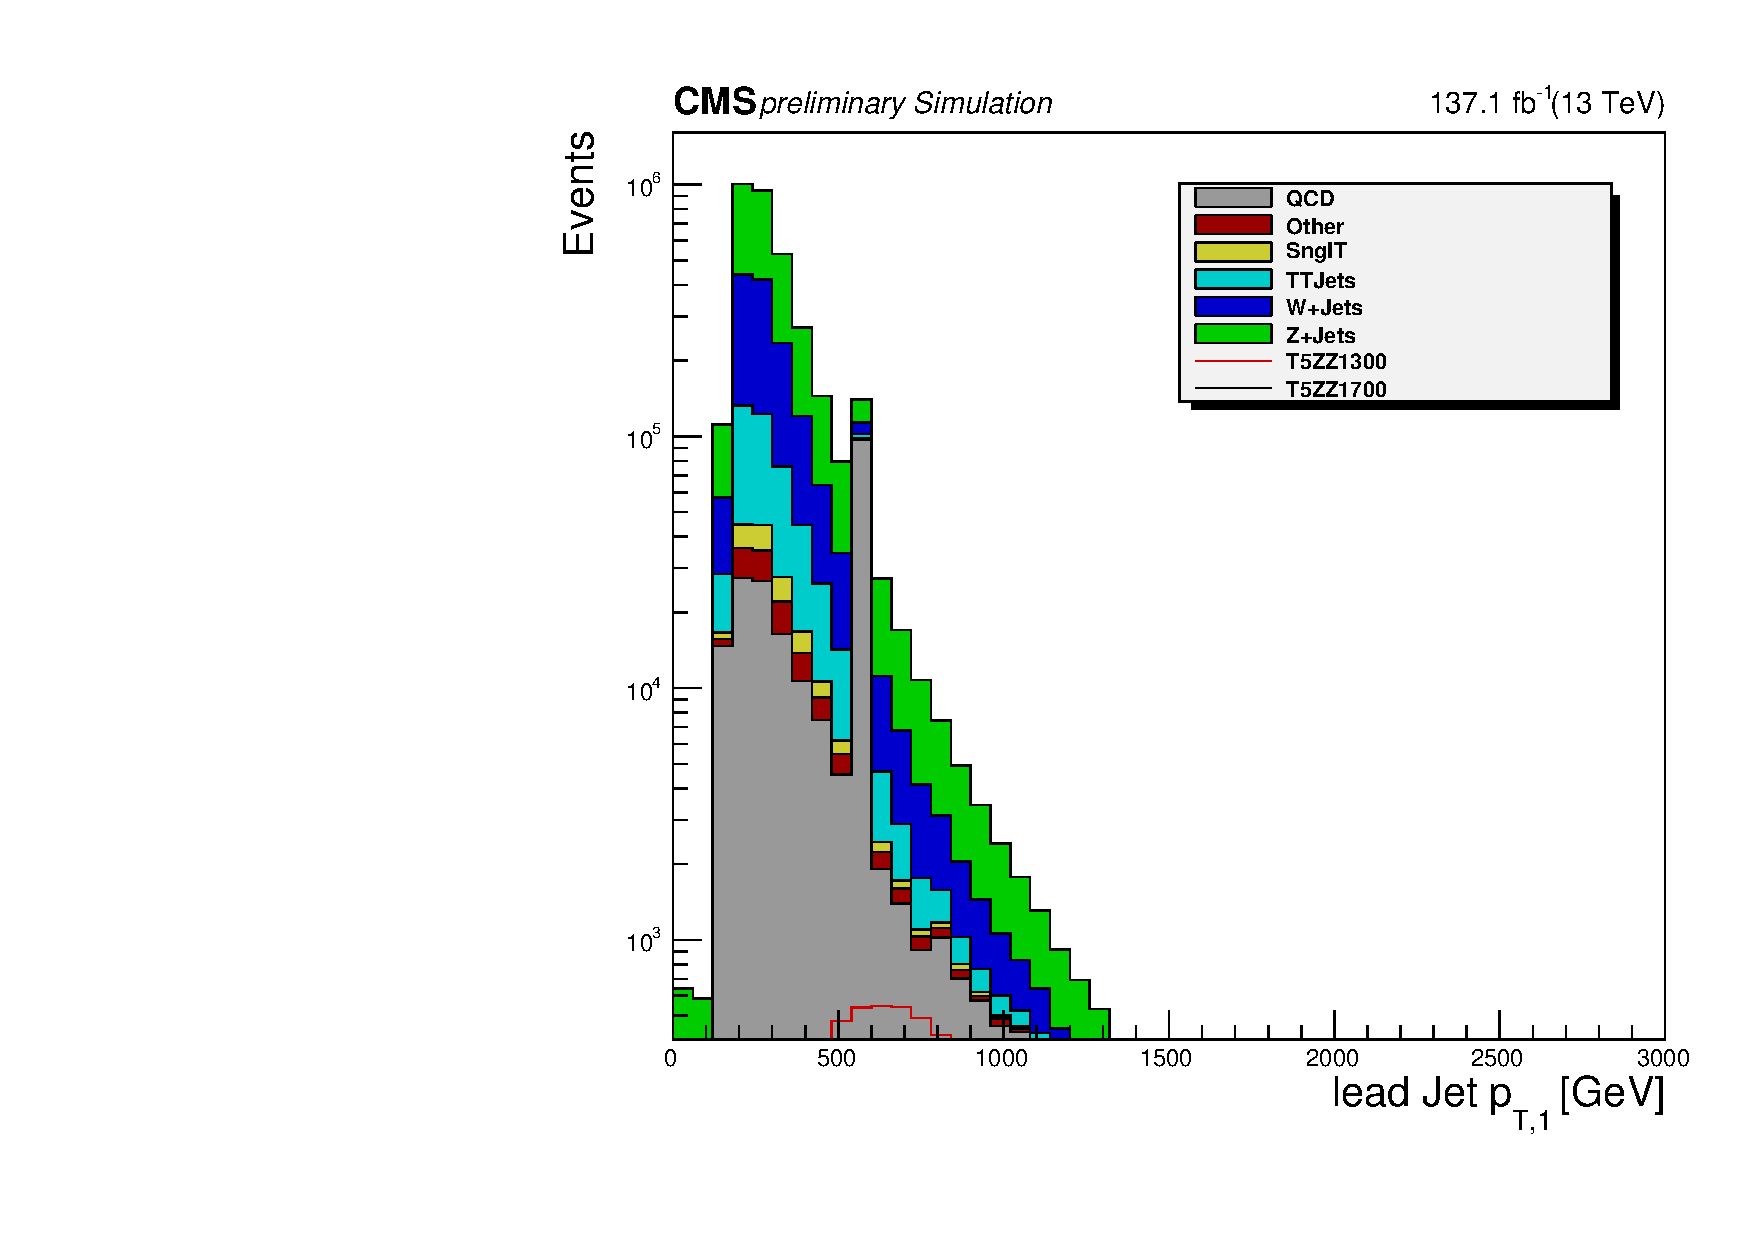
\includegraphics[width=0.48\linewidth]{plots/event-selection/2017JetPt1scaled137_baseline.pdf}
  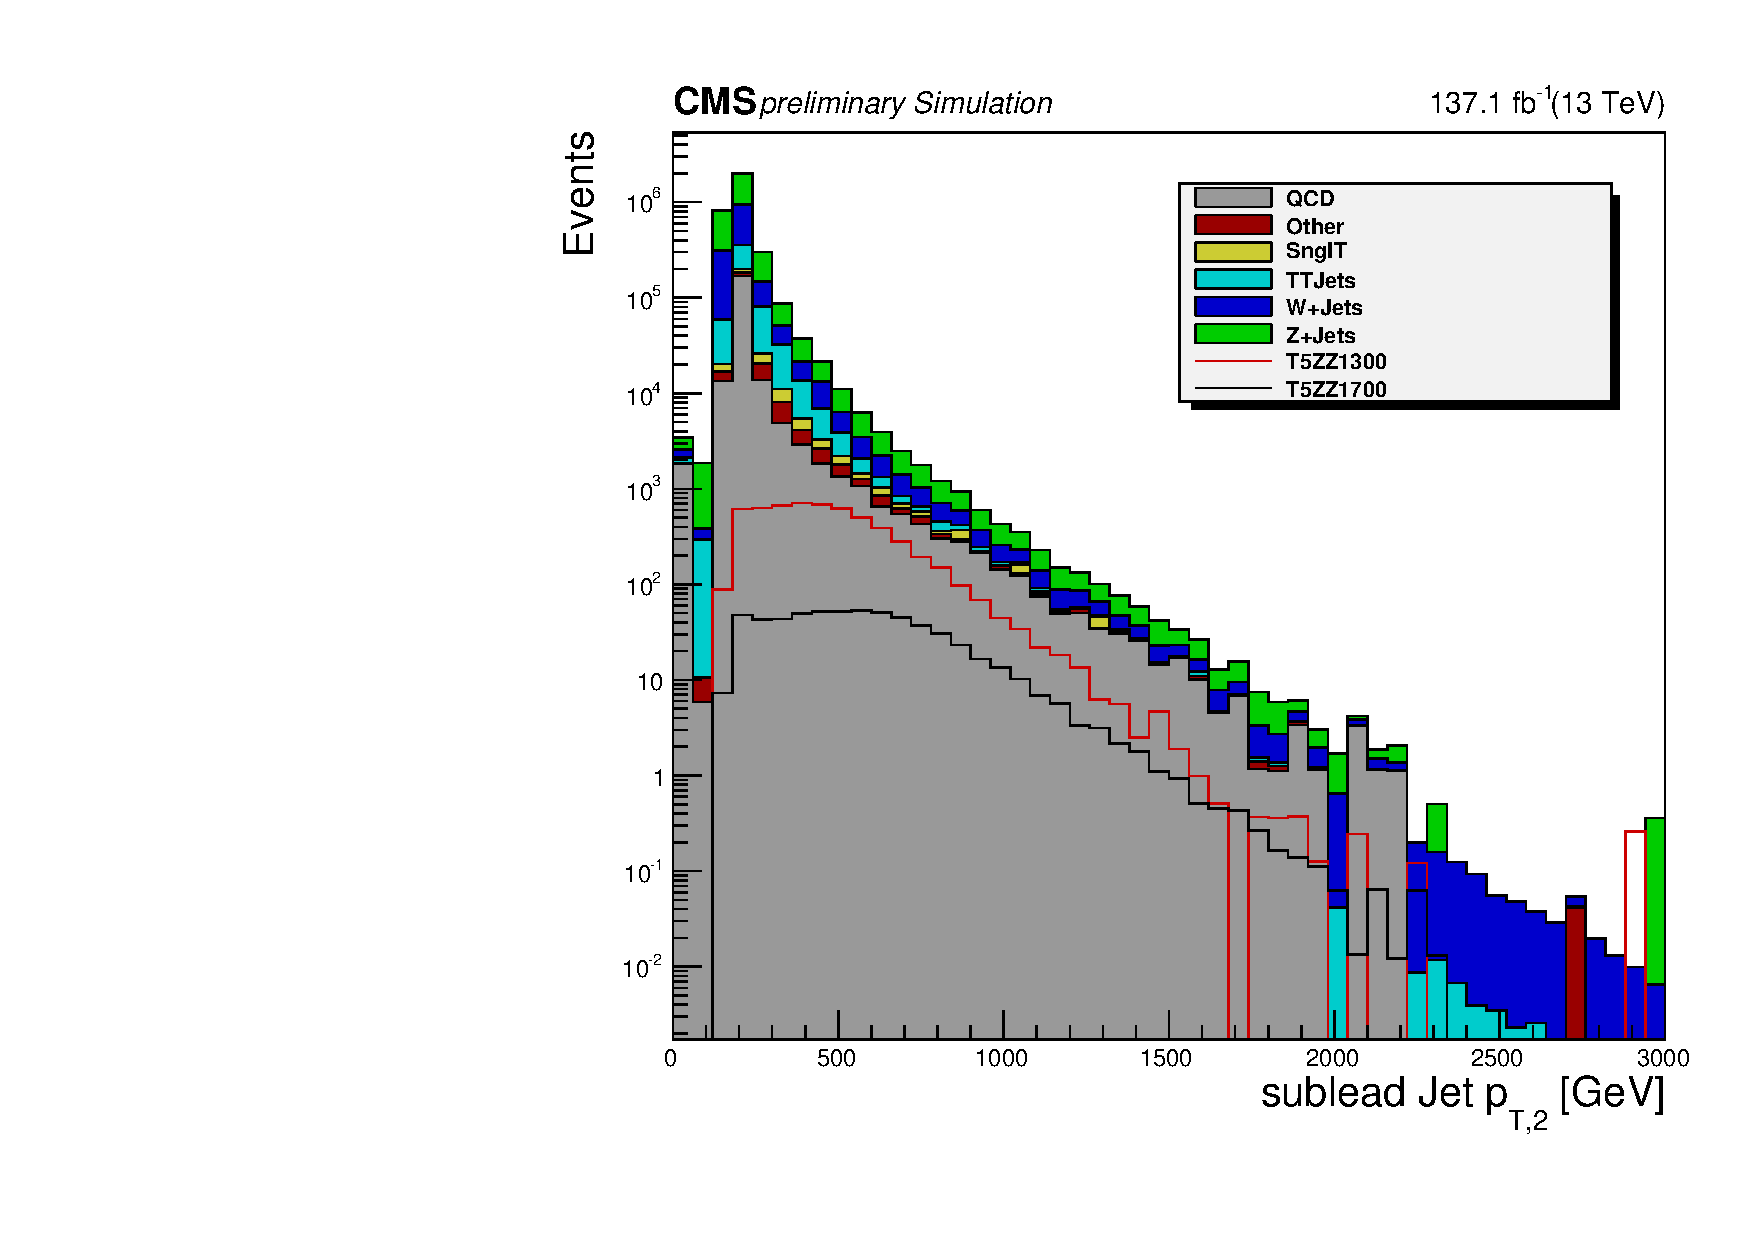
\includegraphics[width=0.48\linewidth]{plots/event-selection/2017JetPt2scaled137_baseline.pdf}\\[1mm]
  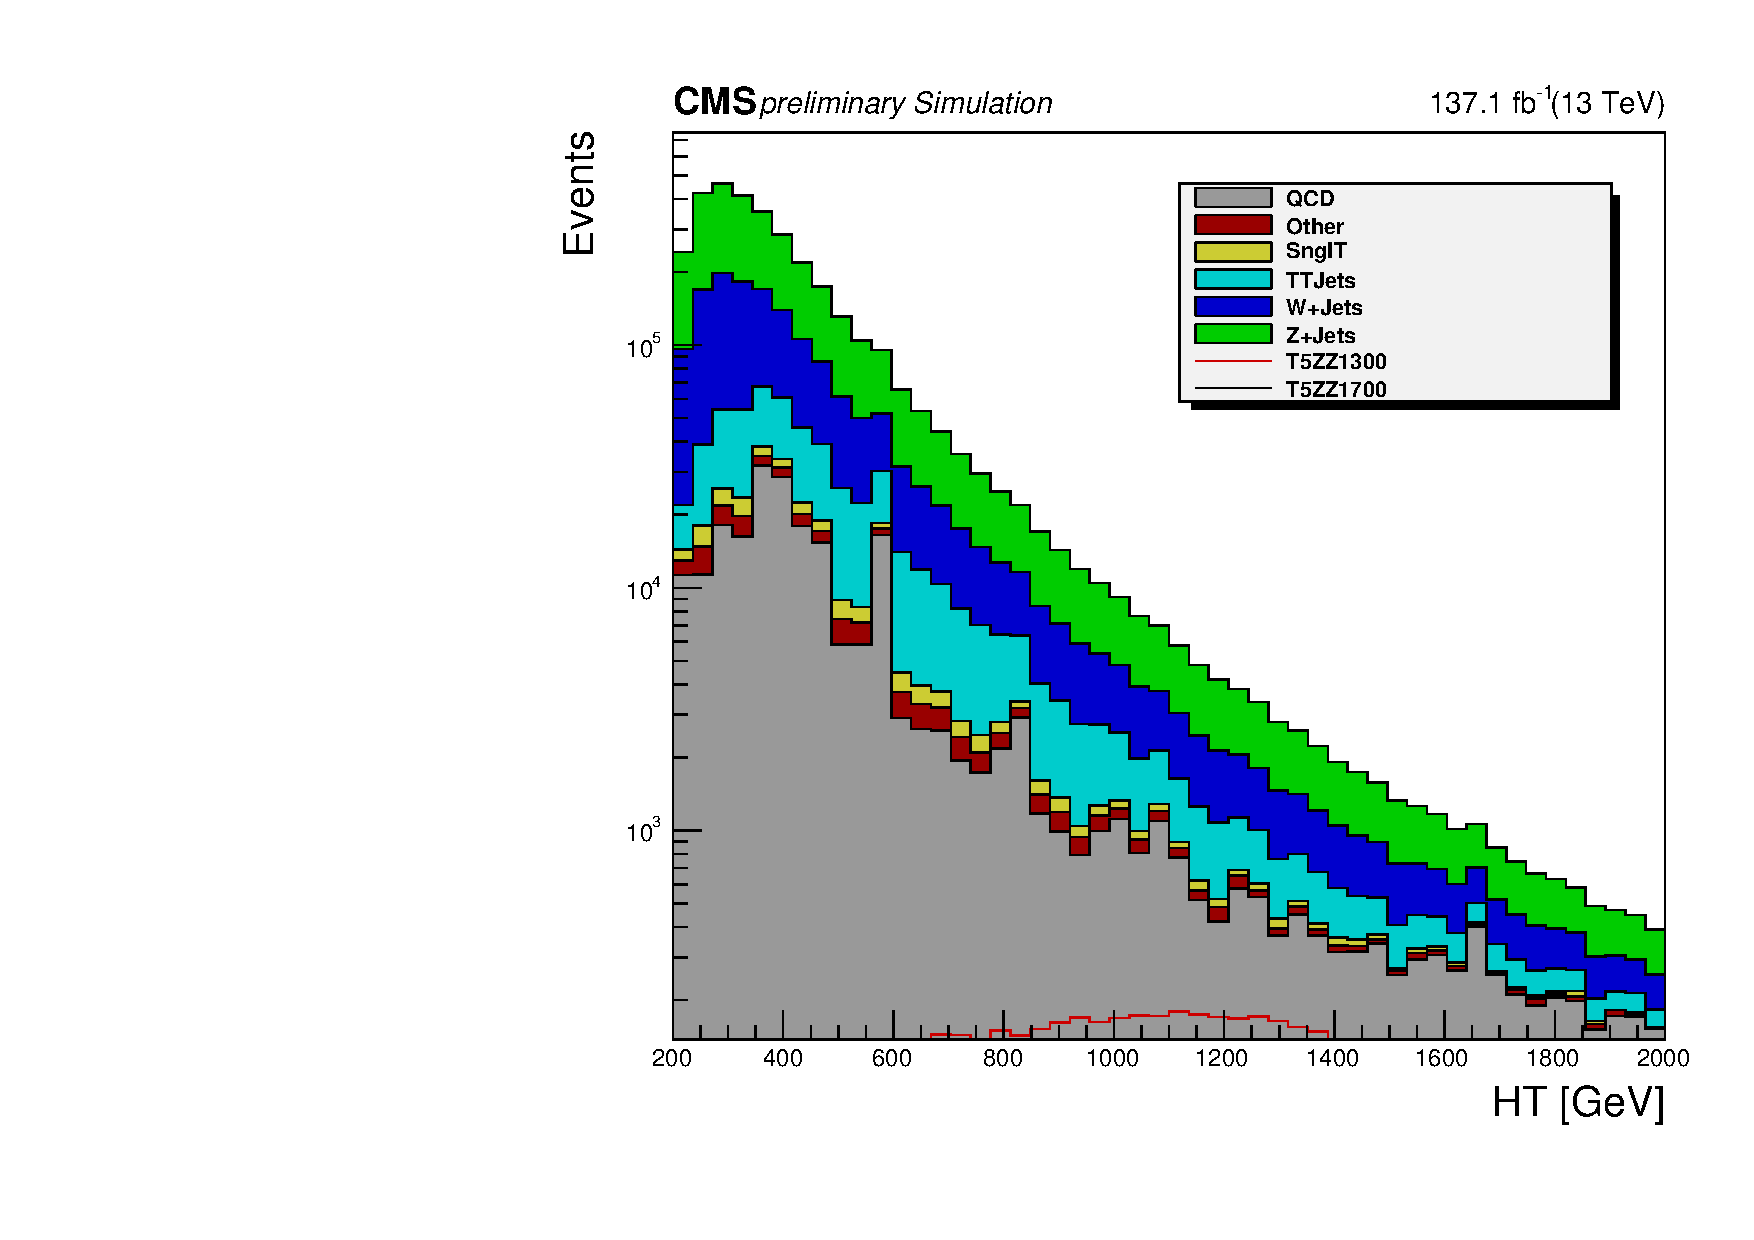
\includegraphics[width=0.48\linewidth]{plots/event-selection/2017HTscaled137_baseline.pdf}
  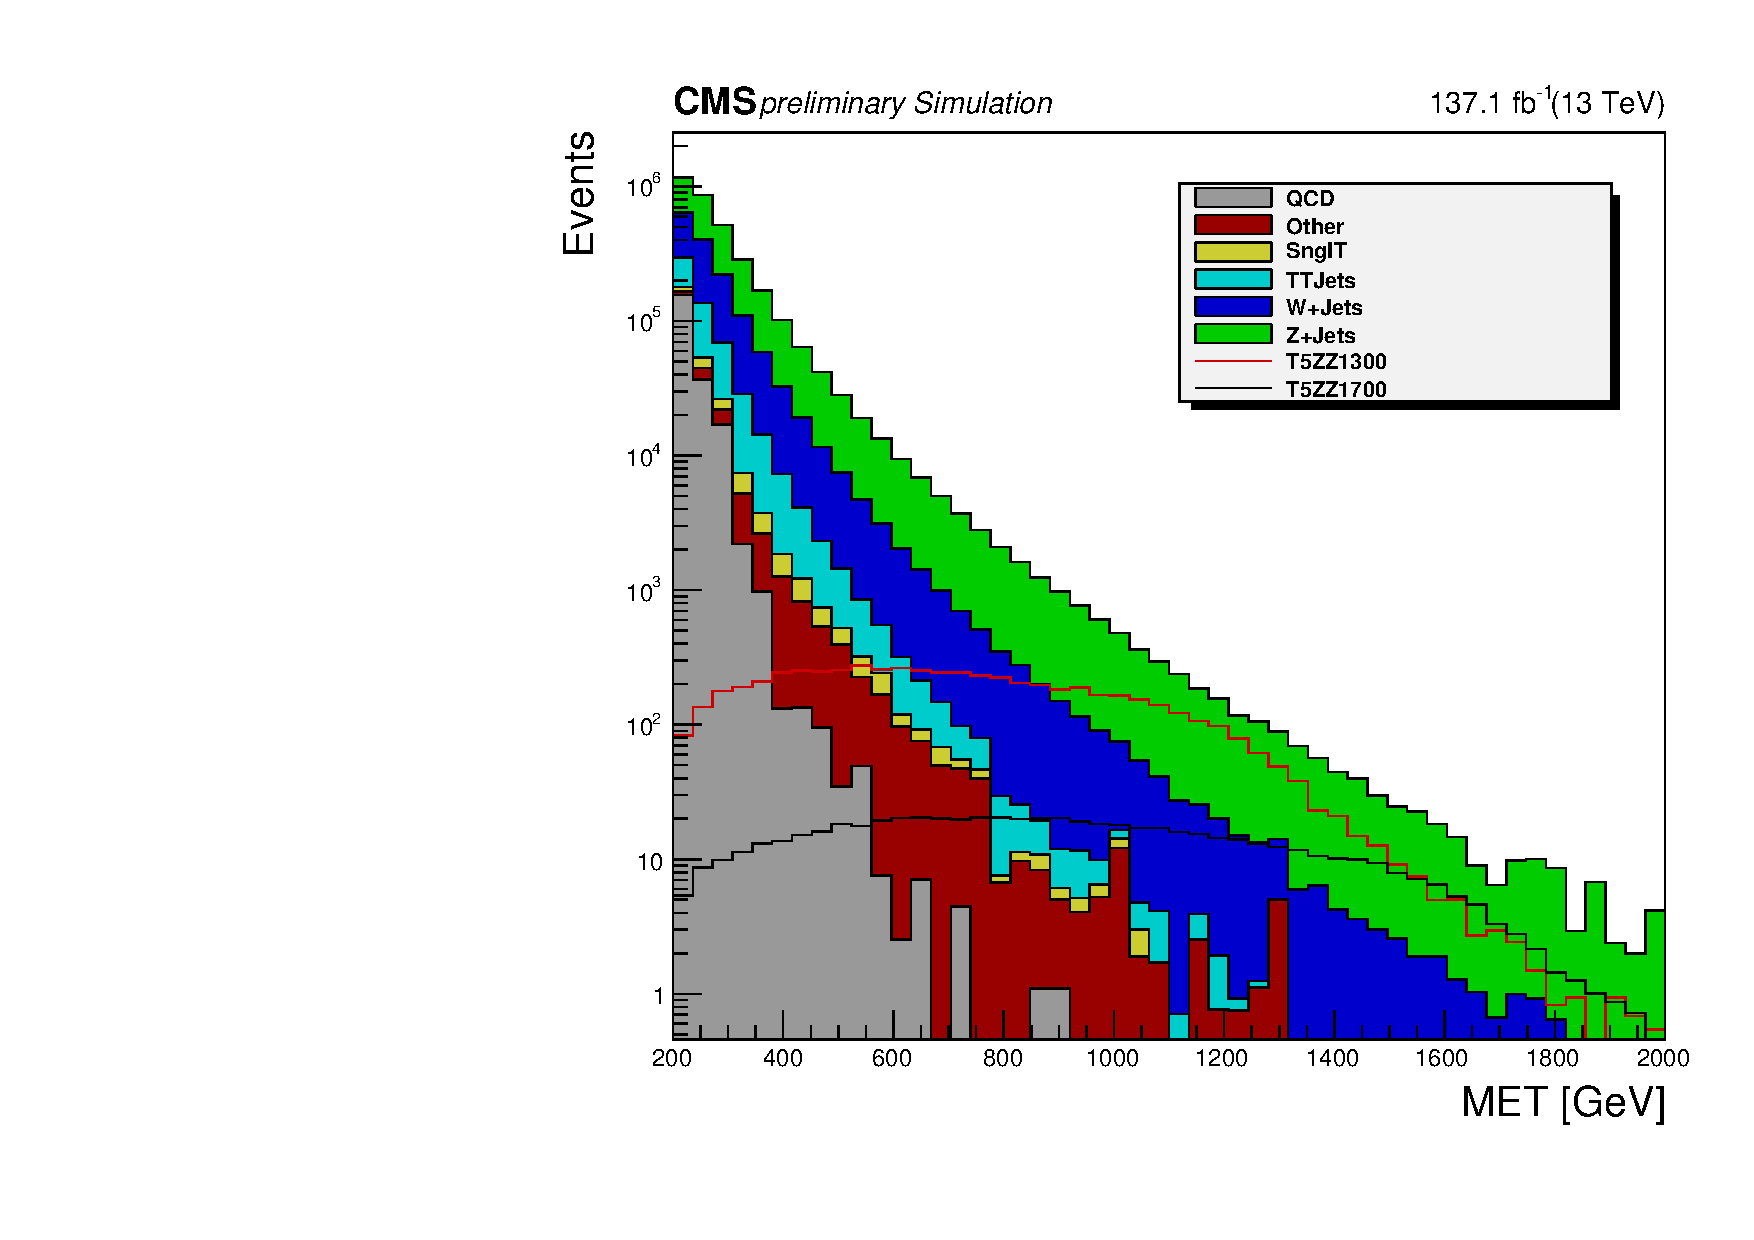
\includegraphics[width=0.48\linewidth]{plots/event-selection/2017METscaled137_baseline.pdf}\\[1mm]
 % \includegraphics[width=0.48\linewidth]{plots/event-selection/.pdf}
 % \includegraphics[width=0.48\linewidth]{plots/event-selection/.pdf}\\[1mm]
  \caption{
     Top: Jet \pt distributions after baseline selection except \HT,\MET, $\delta$R, jet mass and \pt requirements.
     Bottom:  \HT(left) and \MET(right) distributions after  baseline selection except \HT,\MET, $\delta$R, jet mass and \pt requirements.
  }
  \label{fig:cutFlow}
\end{figure}

\begin{figure}[htbp!]
  \centering
  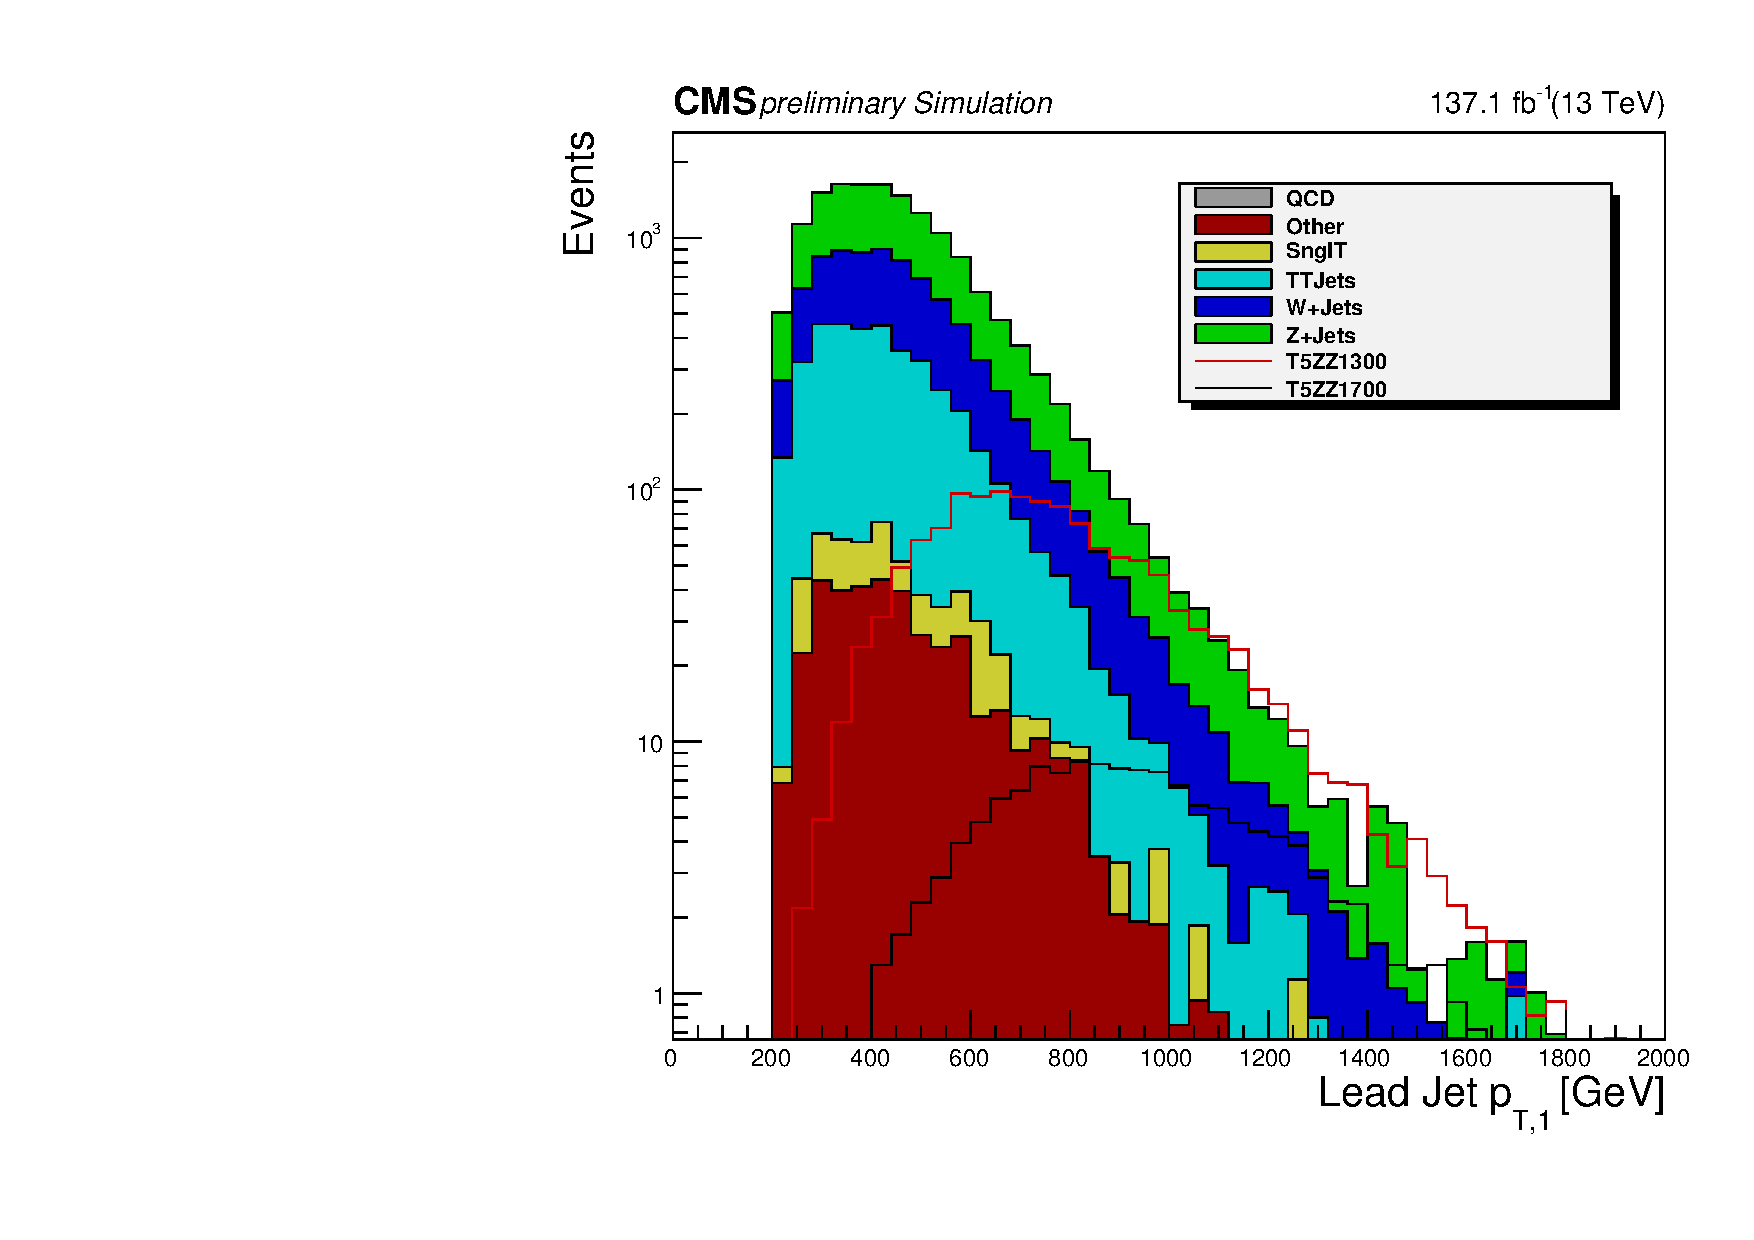
\includegraphics[width=0.48\linewidth]{plots/event-selection/JetPt1scaled137_selection.pdf}
  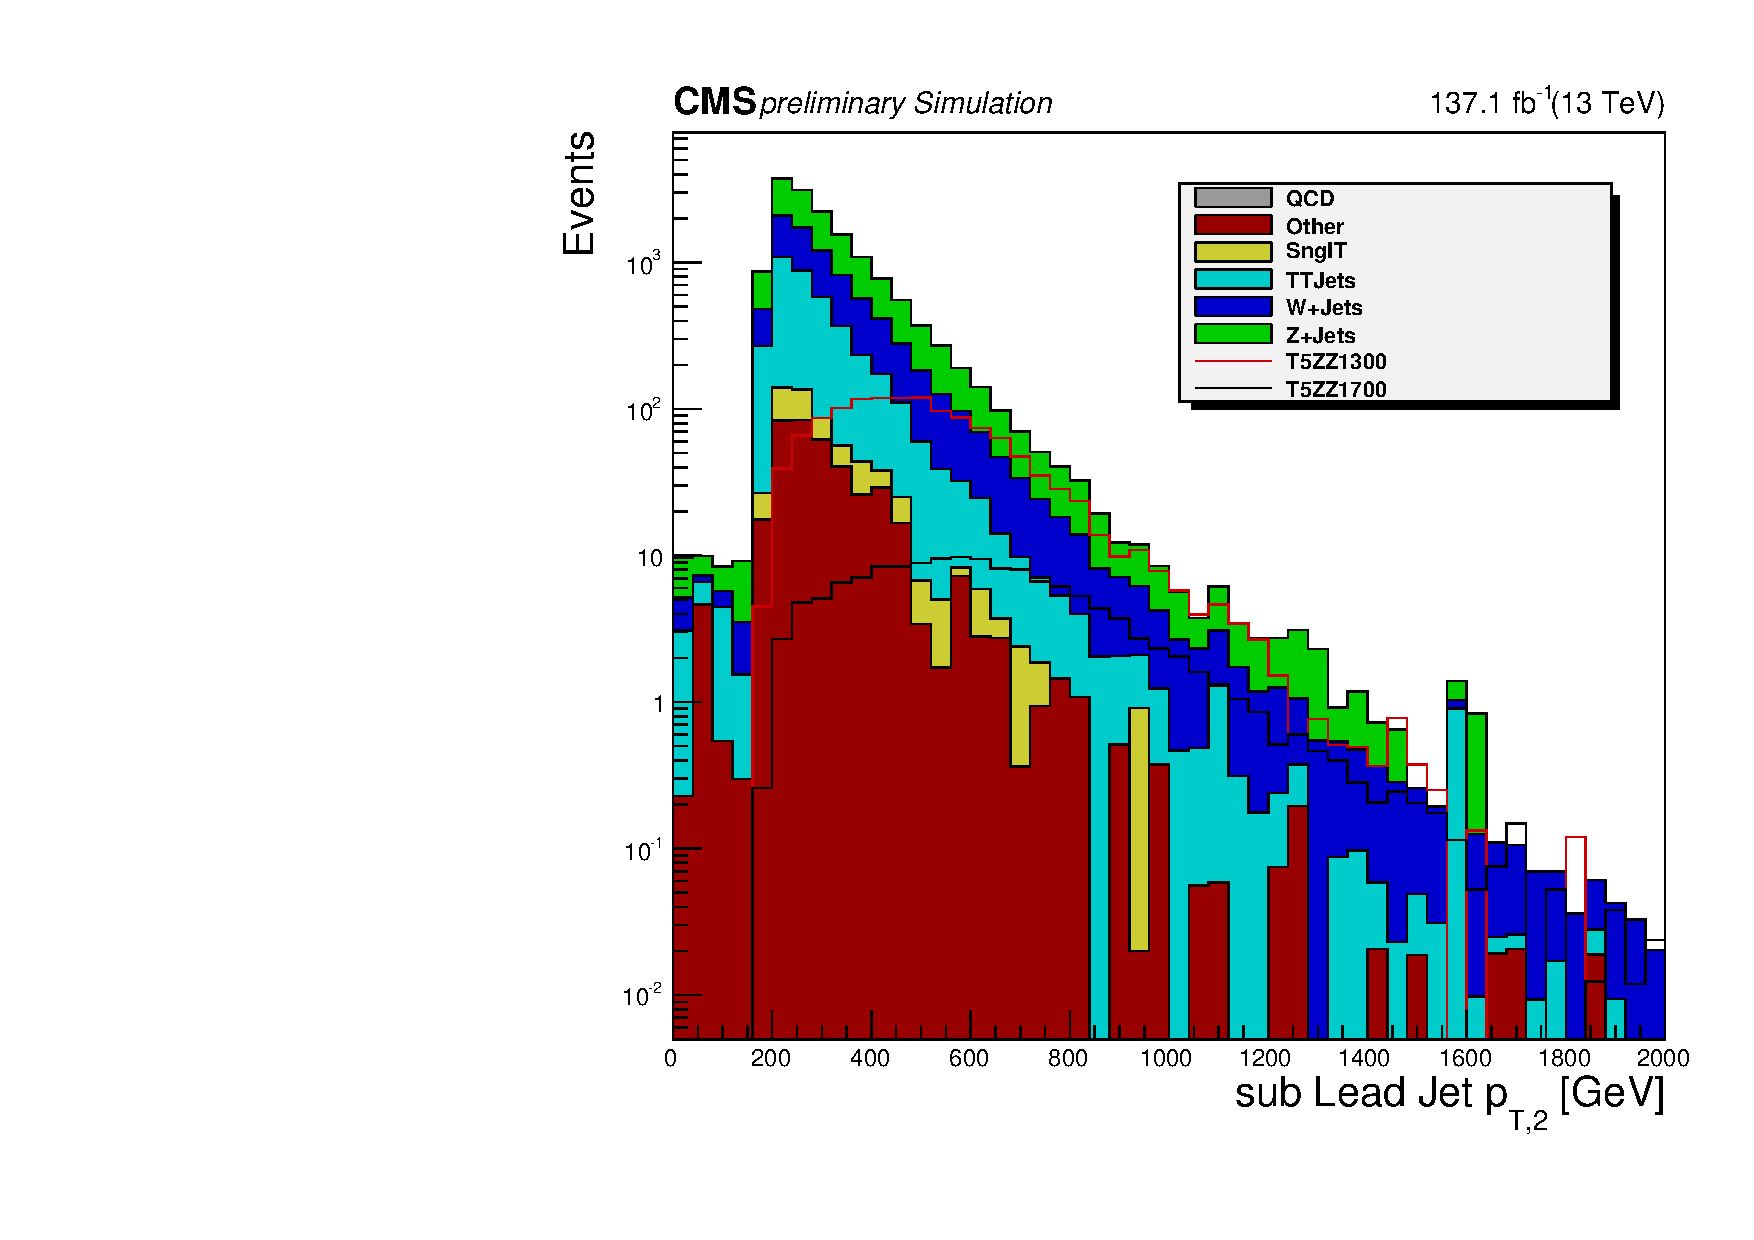
\includegraphics[width=0.48\linewidth]{plots/event-selection/JetPt2scaled137_selection.pdf}\\[1mm]
  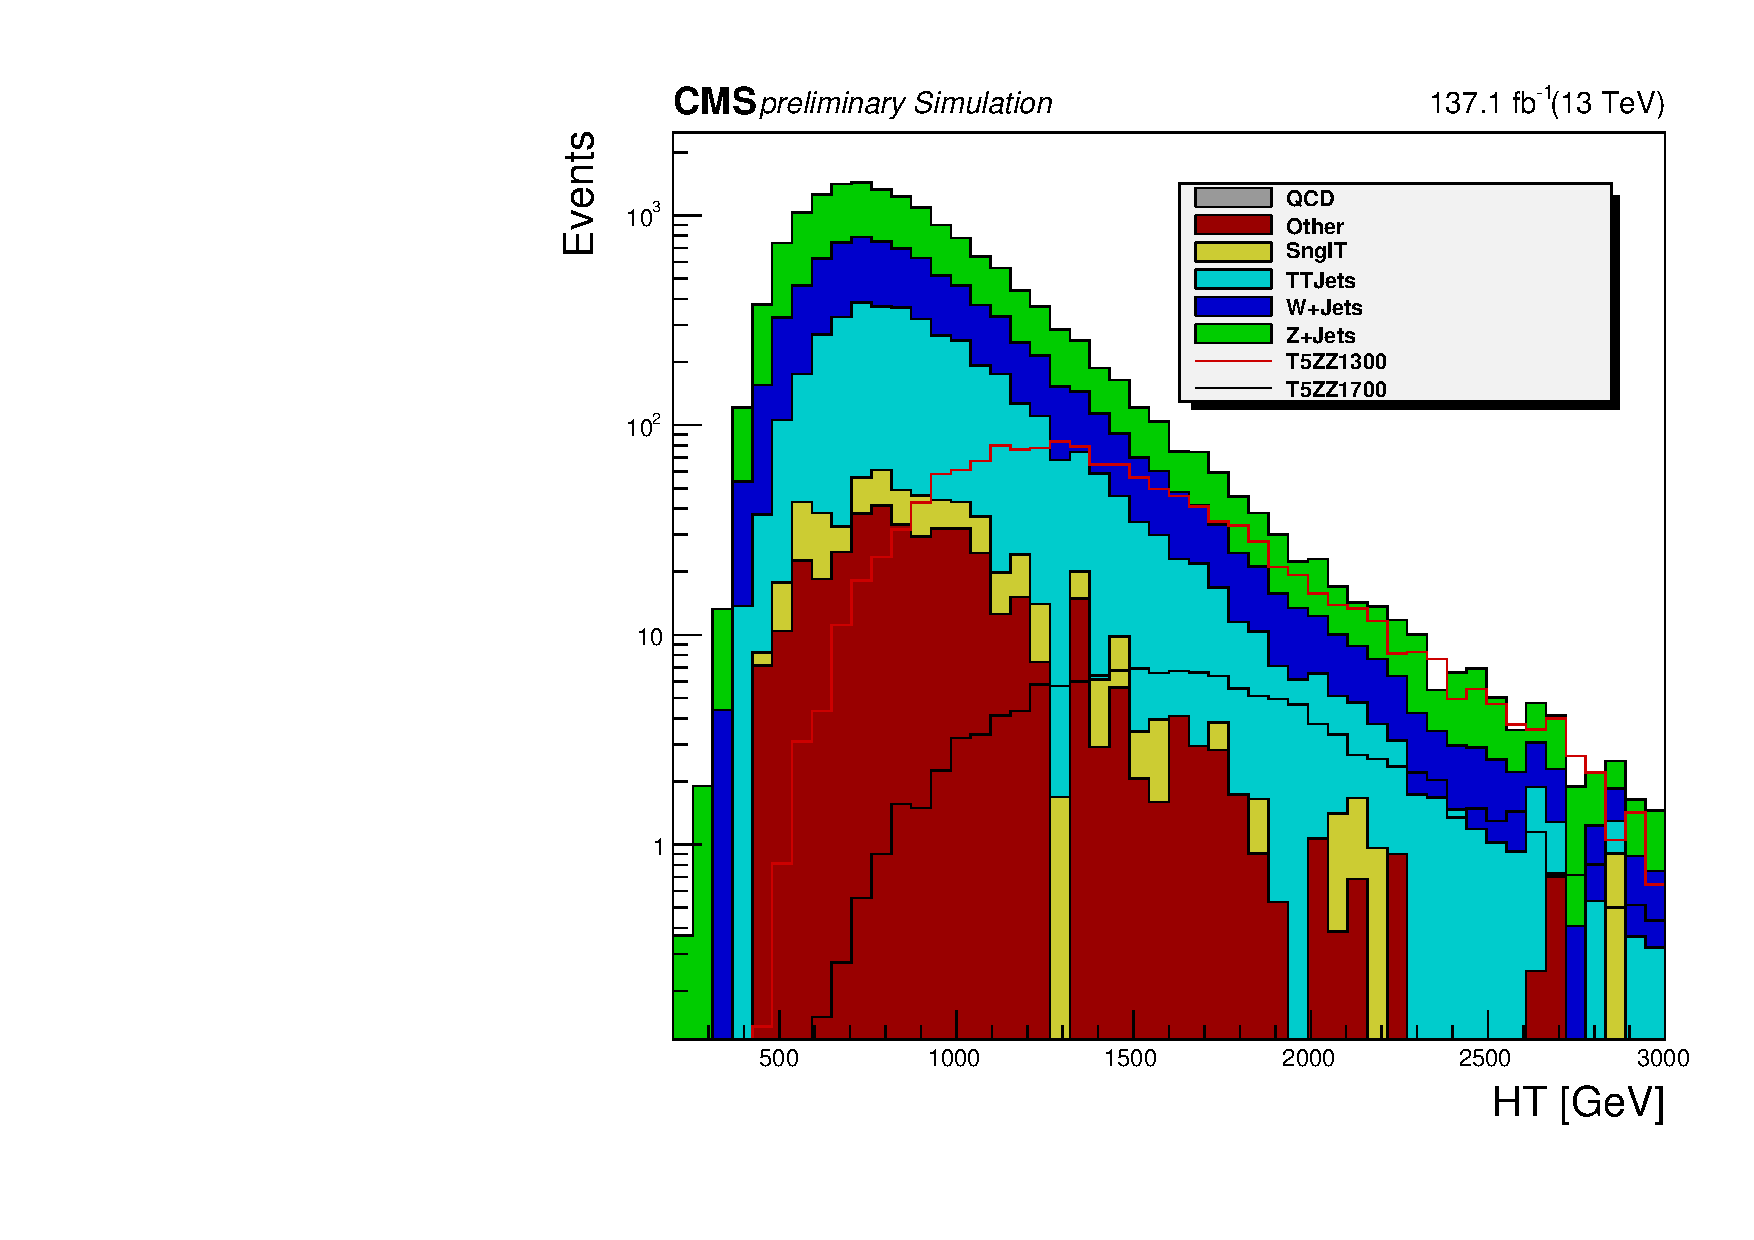
\includegraphics[width=0.48\linewidth]{plots/event-selection/HTscaled137_selection.pdf}
  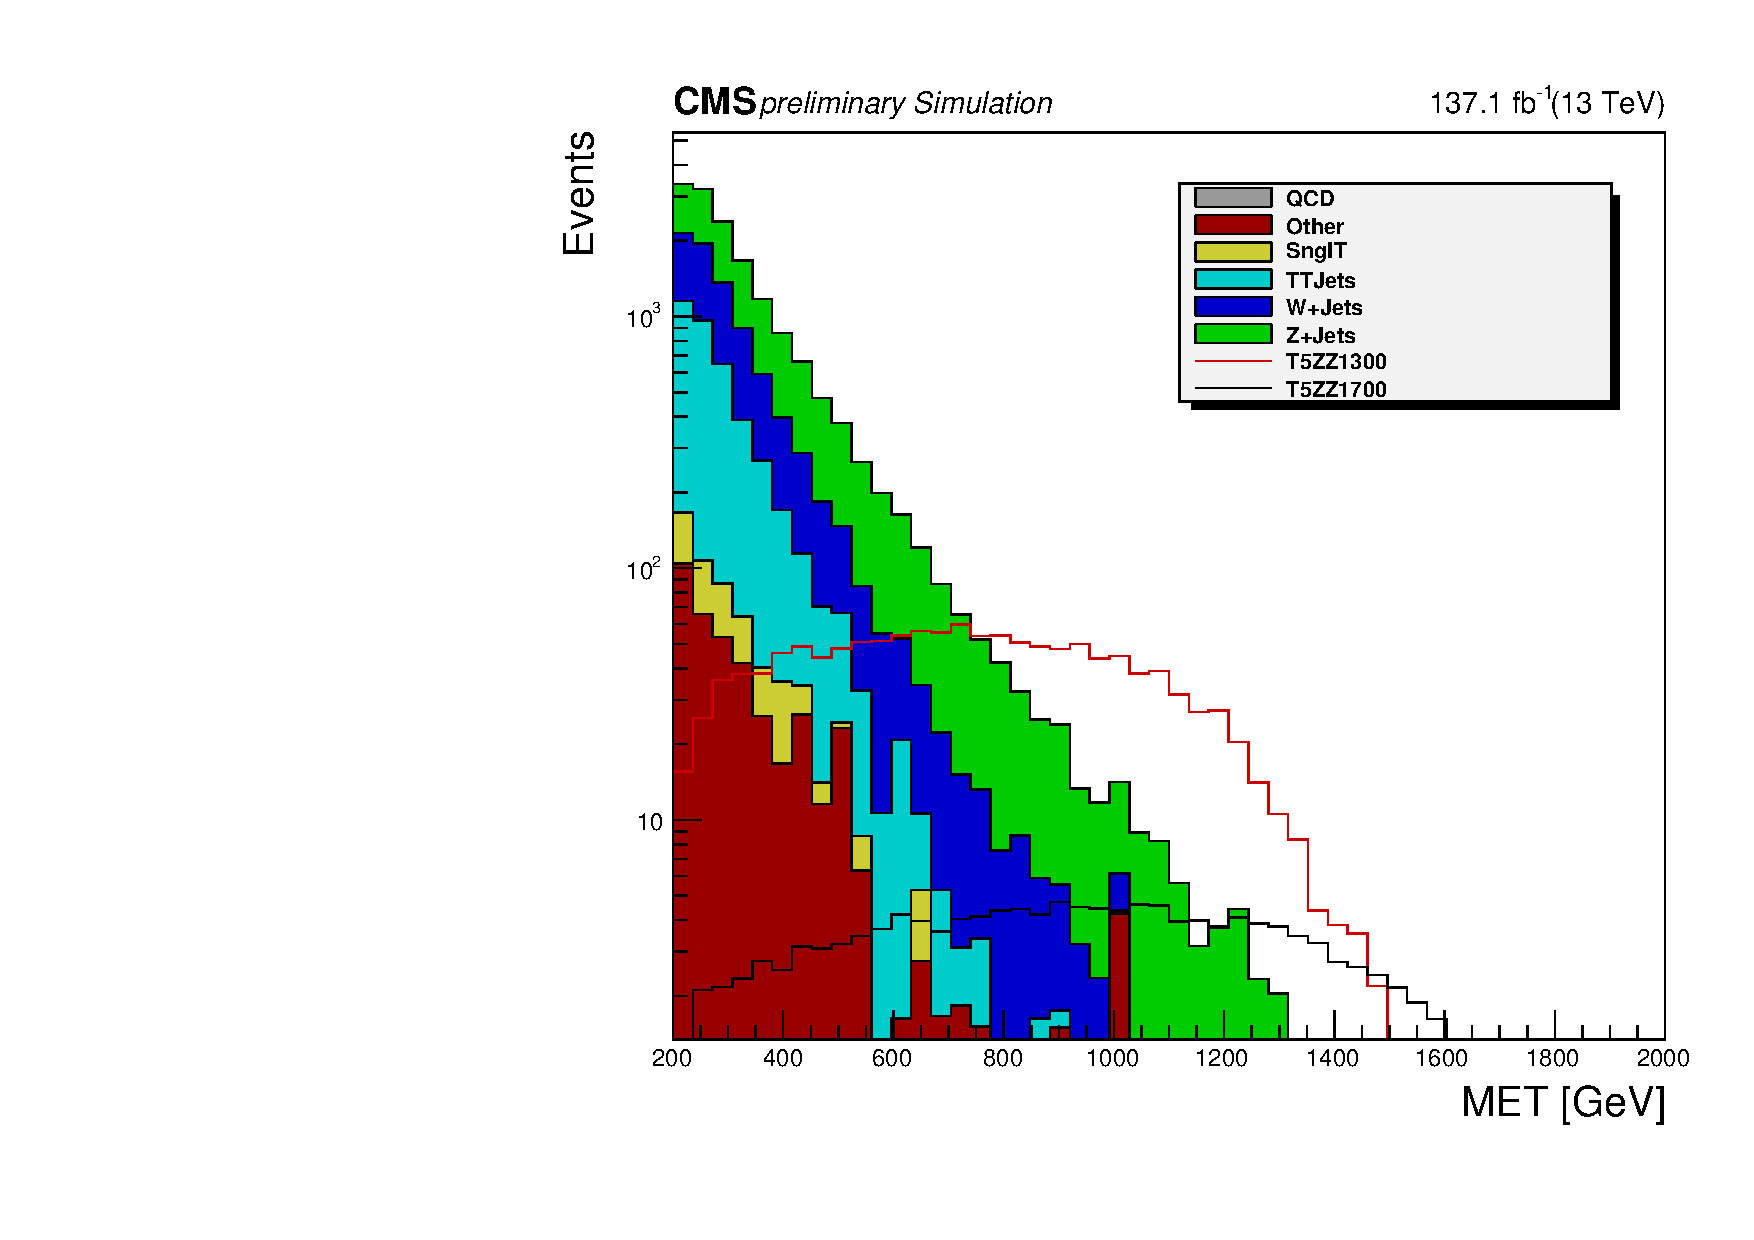
\includegraphics[width=0.48\linewidth]{plots/event-selection/METscaled137_selection.pdf}\\[1mm]
  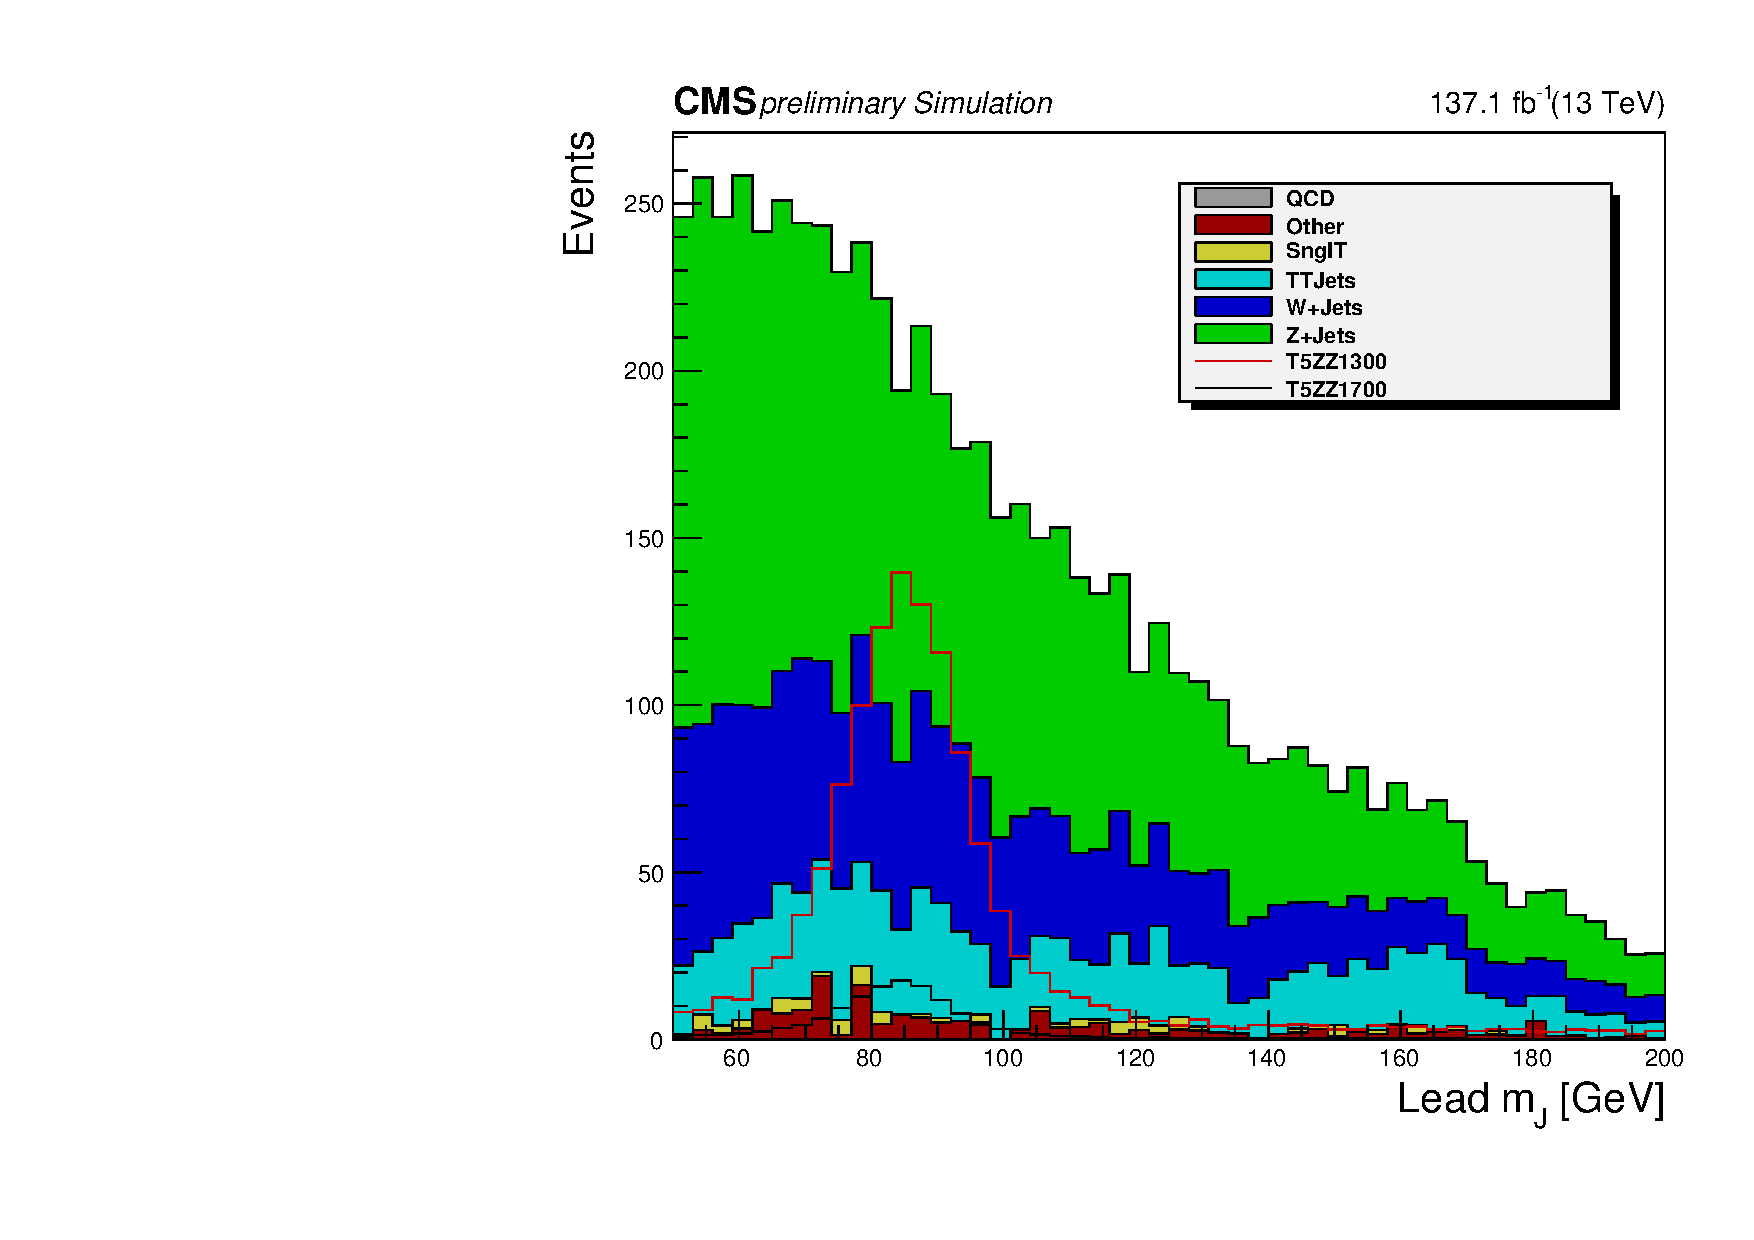
\includegraphics[width=0.48\linewidth]{plots/event-selection/PrunedMass1scaled137allselection.pdf}
  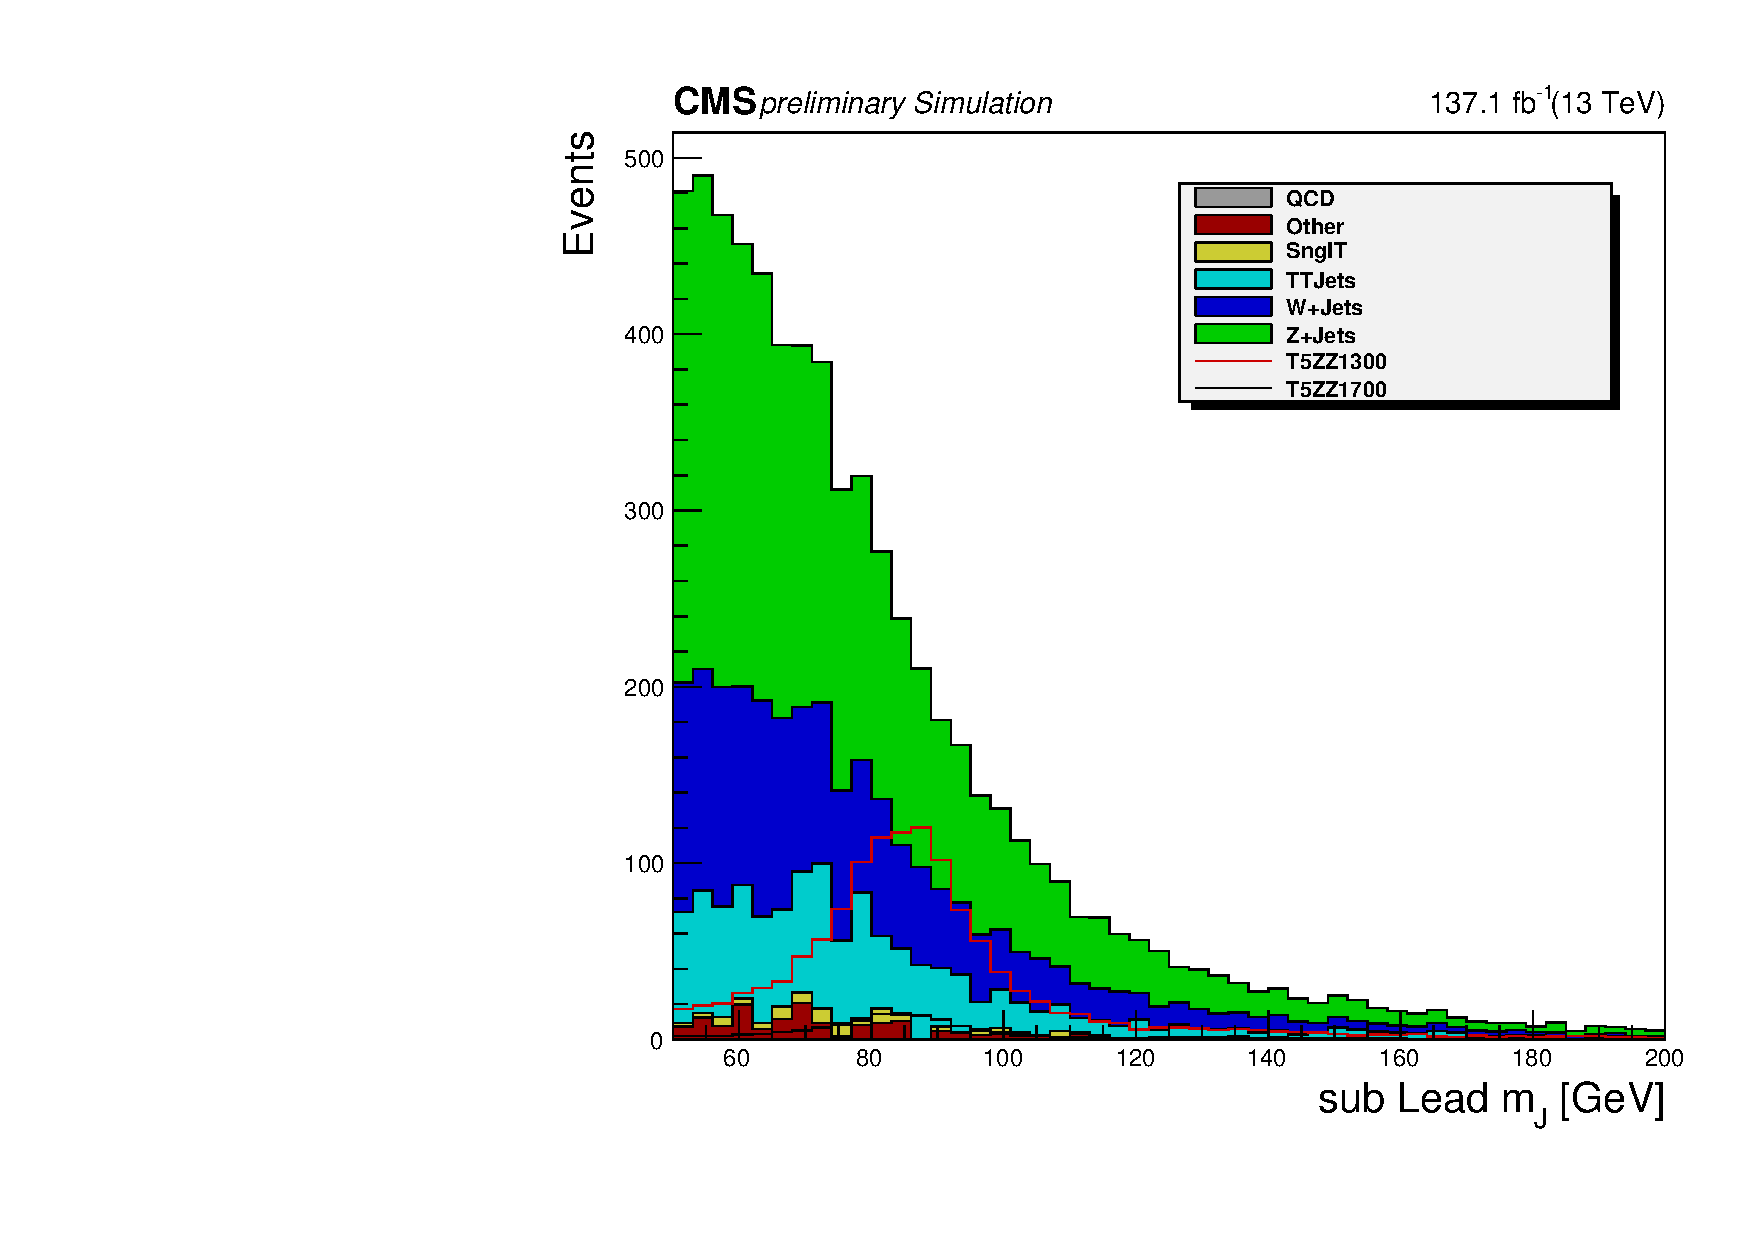
\includegraphics[width=0.48\linewidth]{plots/event-selection/PrunedMass2scaled137allselection.pdf}\\[1mm]
  \caption{
     Top: Jet \pt distributions after baseline selection except \HT,\MET and \pt requirements.
     Center:  \HT(left) and \MET(right) distributions after  baseline selection except \HT,\MET and \pt requirements.
     Bottom: Softdrop jet mass distributions after  baseline selection.
  }
  \label{fig:cutFlow2}
\end{figure}


\newpage
\begin{landscape}
 \begin{table}[htb!]
  \caption{
   Cut flow table for each of the main MC background samples and their sum. The table also includes the signal for two mass points of the 2Z final state. Cuts on the AK8 jets are applied to both the leading and subleading jets.
  }
  \begin{tabular}{|c|c|c|c|c|c|c|c|}
   \hline
	\hline
   Cut & Total Bkg. & $Z\rightarrow\nu\nu$ & $W\rightarrow\ell\nu$ & $t\overline{t}$ & QCD & T5HH1300 & T5HH1700  \\
	\hline
	\hline
	\multicolumn{8}{c}{Baseline SUSY Hadronic Skim: $\met>300\gev$, $HT>300\gev$, $\Delta\phi$ cuts, Lepton Veto, Isolated Track Veto}\\
   \hline
	Baseline SUSY Hadronic Skim &  439015 & 293825 & 118287 & 26121 & 780 & 1550  & 169 \\ \hline
	$\met>300\gev$ & 112300 & 69855 & 26868 & 14806 & 769 & 1525 & 159.4 \\ \hline
	$HT>500\gev$ & 46153 & 26409 & 10661 & 8627 & 455.8 &  1486 & 159.4 \\ \hline
	AK8 Lead Jet $\pt>300\gev$ &  42321  & 24672 & 9835 & 7502 & 310.1 & 1342  & 143.9 \\ \hline
	AK8 subLead Jet $\pt>200\gev$ & 29577  & 17428 & 6935.5  & 4940.7 &  272.5& 1183  & 128 \\ \hline
	AK8 Jet Mass in $[50,200]\gev$ & 6107.8 & 2964.8 & 1292.1 & 1789.1 &61.7 &   785 &  86   \\ \hline
	$\Delta$ R $>$ 0.8 for sublead AK8 Jet &2478 & 1400 & 668.3 & 378.7 &31 & 402 & 44  \\ \hline
	AK8 Jet Mass in $[70,100]\gev$ &  284.1 & 161 & 78.8 & 42.8 & 1.37 & 229 & 28\\ \hline
   \hline
   \hline
   \end{tabular}
   \label{tab:Cutflow}
  \end{table}
\end{landscape}

\subsection{Signal Regions}

\begin{figure}[htbp!]
  \begin{center}
    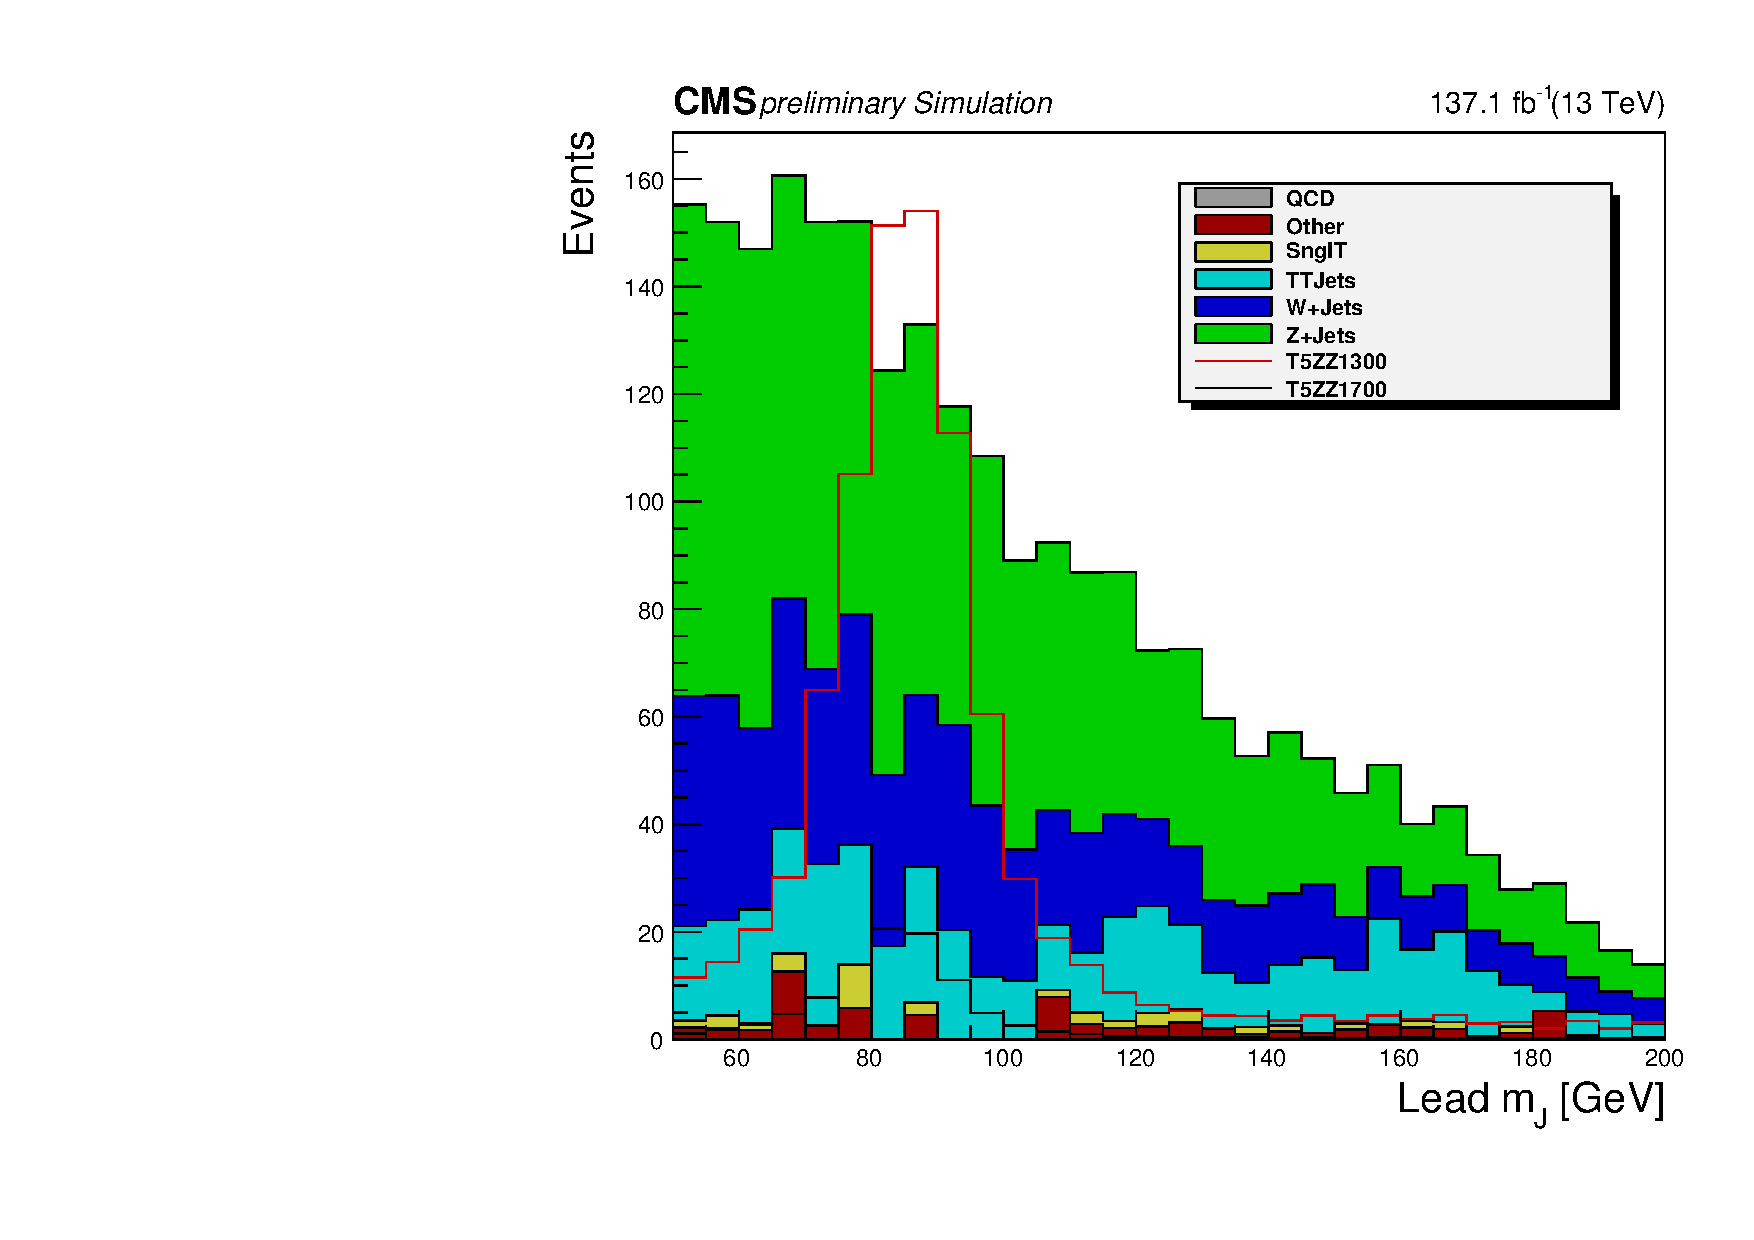
\includegraphics[trim={5px 5px 5px 5px},clip,width=0.48\linewidth]{plots/event-selection/PrunedMass1scaled137_fitting.pdf}
    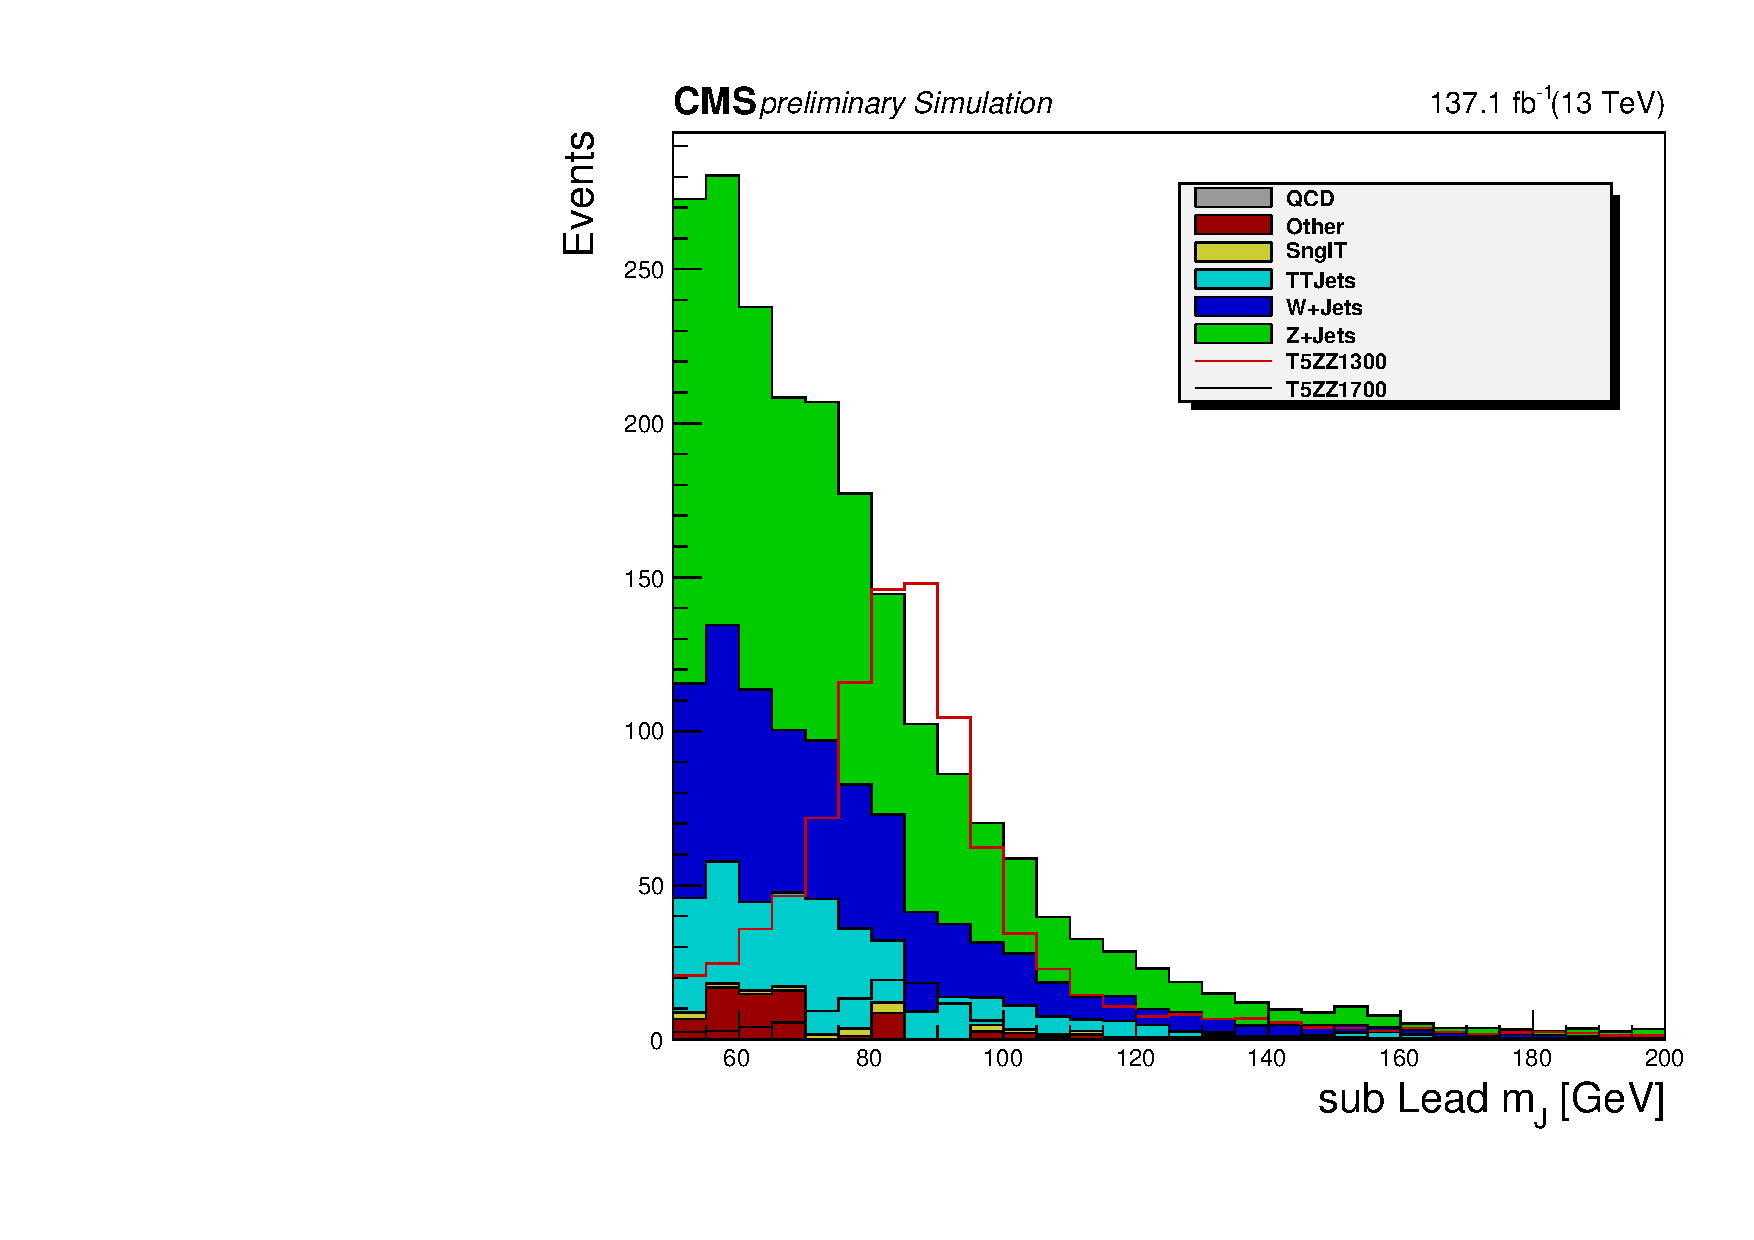
\includegraphics[trim={5px 5px 5px 5px},clip,width=0.48\linewidth]{plots/event-selection/PrunedMass2scaled137_fitting.pdf}
    \caption{
      Distribution of the leading (left) and subleading (right) AK8 pruned-jet mass after the baseline selection, for leading jet baseline selections are all but lead jet mass[50,200] and for sublead jet vice-versa.
    }
    \label{fig:JetMass_baseline}
  \end{center}
\end{figure}


\subsection{Control Regions}

